\documentclass[../main.tex]{subfiles}

\graphicspath{{ima/clase10}{ima}}

% Aquí empieza el documento{{{
\begin{document}

\chapter{Conteo}%

\thispagestyle{fancy}

\begin{align*}
	[n] = \{x\in\mathbb{N}:x\leq n\}\\
	f:[m]\longrightarrow[n]\\
	m.n\in\mathbb{B}
\end{align*}

Cuantas \underline{funciones totales} hay.



Hay $n^m$ funciones totales posibles ente $[m]$ y $[n]$.
\begin{align*}
	m &=4 && f:[4]\longrightarrow[3]\\
	n &=3
\end{align*}

\begin{center}
	\begin{tabular}{c|c|c|c|c}
		$[m]$ & $f_1$ & $f_2$ & $f_3$ & \\
		\hline
		1 & 1 & 2 & 3 & 1\\
		2 & 1 & 1 & 1 & 2\\
		3 & 1 & 1 & 1 & 1\\
		4 & 1 & 1 & 1 & 1\\
	\end{tabular}
\end{center}

De cuántas formas podemos pintar una madera
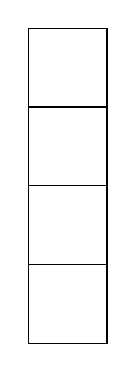
\begin{tikzpicture}[scale=1, transform shape]
	\draw (0,0) -- ++(1,0)
		-- ++(0,-4)
		-- ++(-1,0)
		-- (0,0)
		;
	\foreach \ii in {-1,...,-3}
	{
		\draw (0,\ii) -- ++(1,0);
	}
\end{tikzpicture}
usando los colores rojo, azul, verde en los rectángulos marcados.
Todos los rectángulos de la cara frontal deben estar pintados.

$3^4$
Porque hay $4$ casilleros y $3$ opciones.

¿De cuantas maneras se puede pintar la anterior madera antes de clavar la base?
\begin{align*}
	\intertext{ $3^4$ es el resultado anterior, $3^2$ son los que no
	tienen duplicados y $3^4-3^2$ es el número de patrones duplicados}
	%\frac{3^4-3^2}{2}  +3^2 = 45
	\frac{\overbrace{3^4-3^2 }^{\substack{\text{Patrones}\\\text{duplicados}} }}{2}
	\overbrace{+3^2}^{\substack{\text{Patrones}\\\text{irrepetibles}} } = 45
\end{align*}
Lo de arriba es la cantidad de patrones duplicados por 2 más la cantidad de patrones
irrepetibles.

Usando las letras A,B,C cuantas palabras de $4$ letras podemos hacer si una palabra,
es equivalente a su \textcolor{red}{ \textbf{Reversa.}}
\begin{align*}
	\text{ABBA} \cong \text{ABBA}\\
	\text{CABA} \cong \text{ABAC}
\end{align*}
{\Huge\[45\]}

\teorema
{
	\Huge
	\begin{align*}
		f:A\longrightarrow B &&\text{y $f$ es |:| (Biyección total)}\\
		|A| = |B|
	\end{align*}
}
\begin{align*}
	R &= \{(x,y)\in\mathbb{N}^2:x\leq y\}\\
	S &= R \cup\{(x,\infty):x\leq\mathbb{N}\}\\
	S &= R \cup\{(\infty,\infty)\}\\
	\Big{(}
	\mathbb{N} \cup \{\infty\},S
	\Big{)}
\end{align*}

\[|A| < \infty\]
$f:A\longrightarrow B$ es total si Dom$f=A$
\begin{align*}
	\text{Si } f:A&\longrightarrow B \text{ es total.}\\
	|B| &\leq |A|
\end{align*}
Sobreyectiva:

$f:A\longrightarrow B$ es total y $\underbrace{k:1}_{\text{$k$ a $1$}}$
$\forall y \in B\ \exists x \in A\ f(x)=y$
\teorema
\textbf{Regla del cociente}
\begin{align*}
	\intertext{Si $f$ es $k:1$ podemos decir que}
	\frac{|A|}{k} &= |B|
\end{align*}

\section{Perdí mis apuntes de discretas I}%
\label{sec:Perdí mis apuntes de discretas I}

Una relación $R\subseteq A\times B$ es una función y
$\Longleftrightarrow(x,y)\in R \wedge (x,y_2)\in R \Longrightarrow y_1=y_2$
\textcolor{red}{ \textbf{De los elementos de $\mathbf{A}$ que salen flechas sale
a los mucho {\Huge $1$} flecha.}}

Una función $f:A\longrightarrow B$ es una relación entre $A$ y $B$
{\Huge
	\begin{align*}
		\text{Dom}f&=\{x\in A:(x,y)\in f\}\subset A\\
		\text{Rango}f&=\{y\in A:(x,y)\in f\}\subset B
	\end{align*}
}

$f$ es total
\[\text{Si Dom}f=A\]

$f$ es inyectiva si y solo si $\Big{(}f(x_1)=y\wedge f(x_2)=y\Big{)}\Longrightarrow(x_1=x_2)$
\textcolor{red}{ \textbf{Los que reciben flechas reciben a los mucho una flecha}}

$f$ es sobreyectiva si Rango$f=R$

$f$ es la identidad si $A=B$ y $f(x)=x \wedge \forall x\in A$
La identidad es $|:|$

$f$ es constante si $|\text{Rango}(f)|=1$

$f$ es $k$-valuada si $|\text{Ranfo}(f)|=k$

$f$ es una biyección si es inyectiva y sobreyectiva.

$f$ es $|:|$ si es una biyección total.

¿De cuantas formas podemos ordenar $n$ objetos distintos en una fila de $n$ objetos?
{\Huge
	\[n!=P_n\text{\small\ permutaciones de $n$}\]
}
\begin{align*}
	\underbrace{n(n-1)(n-2)(n-3)...(3)(2)(1)}_{\text{$n$ factores}}
	= \prod^n_{j=1}j=n!=P_n
\end{align*}

¿De cuantas formas podemos seleccionar $k$ objetos entre $n$ objetos distintos y
ordenarlos en una fila de largo $k$?
\begin{align*}
	\frac{n!}{(n-k)!} = \bigvee^n_k \text{\ variaciones de $n$ en $k$}
\end{align*}
¿De cuántas formas podemos seleccionar $k$ objetos de entre $n$ objetos distintos?
(Creo que es lo anterior pero sin ordenar)

\begin{align*}
	\frac{\bigvee^n_k}{k!}= C^n_k =
	\binom{n}{k}
\end{align*}

\textbf{Calcula usando combinaciones }
\begin{align*}
	&\sum^n_{k=0}\binom{n}{k}\\
	&\sum^n_{k=0}(-1)^k\binom{n}{k}
\end{align*}

\textbf{Solución:}
\[
	\sum_{k=0}^n\binom{n}{k}=2^n
\]
El lado izquierdo cuenta el número de subconjunto de tamaño $k$
de $[n]$ y suma todas las posibilidades para $k$ entre $0$ y $n$

El lado derecho cuenta el número de subconjuntos de $[n]$.
\end{document}
%}}}
